% THIS IS SIGPROC-SP.TEX - VERSION 3.1
% WORKS WITH V3.2SP OF ACM_PROC_ARTICLE-SP.CLS
% APRIL 2009
%
% It is an example file showing how to use the 'acm_proc_article-sp.cls' V3.2SP
% LaTeX2e document class file for Conference Proceedings submissions.
% ----------------------------------------------------------------------------------------------------------------
% This .tex file (and associated .cls V3.2SP) *DOES NOT* produce:
%       1) The Permission Statement
%       2) The Conference (location) Info information
%       3) The Copyright Line with ACM data
%       4) Page numbering
% ---------------------------------------------------------------------------------------------------------------
% It is an example which *does* use the .bib file (from which the .bbl file
% is produced).
% REMEMBER HOWEVER: After having produced the .bbl file,
% and prior to final submission,
% you need to 'insert'  your .bbl file into your source .tex file so as to provide
% ONE 'self-contained' source file.
%
% Questions regarding SIGS should be sent to
% Adrienne Griscti ---> griscti@acm.org
%
% Questions/suggestions regarding the guidelines, .tex and .cls files, etc. to
% Gerald Murray ---> murray@hq.acm.org
%
% For tracking purposes - this is V3.1SP - APRIL 2009

\documentclass{acm_proc_article-sp}

\usepackage{caption}
\usepackage{soul}
\usepackage{color}
\usepackage{url}
\usepackage{hyperref}
\usepackage{subfig}
\usepackage{graphicx}

\begin{document}
\title{Nucleotide Frequencies in the Enterobacteria phage lambda genome}
\subtitle{Assignment 1}
%
% You need the command \numberofauthors to handle the 'placement
% and alignment' of the authors beneath the title.
%
% For aesthetic reasons, we recommend 'three authors at a time'
% i.e. three 'name/affiliation blocks' be placed beneath the title.
%
% NOTE: You are NOT restricted in how many 'rows' of
% "name/affiliations" may appear. We just ask that you restrict
% the number of 'columns' to three.
%
% Because of the available 'opening page real-estate'
% we ask you to refrain from putting more than six authors
% (two rows with three columns) beneath the article title.
% More than six makes the first-page appear very cluttered indeed.
%
% Use the \alignauthor commands to handle the names
% and affiliations for an 'aesthetic maximum' of six authors.
% Add names, affiliations, addresses for
% the seventh etc. author(s) as the argument for the
% \additionalauthors command.
% These 'additional authors' will be output/set for you
% without further effort on your part as the last section in
% the body of your article BEFORE References or any Appendices.

%\numberofauthors{3} %  in this sample file, there are a *total*
% of EIGHT authors. SIX appear on the 'first-page' (for formatting
% reasons) and the remaining two appear in the \additionalauthors section.
%
\numberofauthors{1}
\author{
	\alignauthor Caitlin Ross\\
	\affaddr{Computer Science Department, Rensselaer Polytechnic Institute} \\
	\email{rossc3@rpi.edu}
}
% There's nothing stopping you putting the seventh, eighth, etc.
% author on the opening page (as the 'third row') but we ask,
% for aesthetic reasons that you place these 'additional authors'
% in the \additional authors block, viz.

\date{30 July 1999}
% Just remember to make sure that the TOTAL number of authors
% is the number that will appear on the first page PLUS the
% number that will appear in the \additionalauthors section.

\maketitle

\begin{abstract}
	In order to understand the composition of genomes, the frequencies of each nucelotide in windows can be found.  The frequencies can then be plotted to show areas that are rich in AT or GC content.  This work explores the nucleotide frequences of the Enterobacteria phage lambda genome using three window sizes.  The frequencies of the nucleotides are then plotted for each window.  The frequencies of GC and AT content are also determined for these windows.  The results show that approximately the first 20,000 base pairs are more GC rich, while the rest of the genome tends to be more AT rich.
\end{abstract}


\section{Problem Statement}
The problem is to examine nucleotide frequencies in the Enterobacteria phage lambda genome using various window sizes.  This can be used to look at the composition of the genome and determine which areas are more AT rich and which are more GC rich.  
\section{Methods}
First I downloaded the Enterobacteria phage lambda complete genome from BLAST.  I selected 'Nucleotide' from the database and searched for 'NC\_001416', which is the accession number for this genome.  I downloaded the genome in FASTA format and saved it as lambda.fasta.

Then I wrote a python program to examine the genome composition. The program takes in the lambda.fasta file and then calculates the frequencies of each nucleotide (A, C, G, and T) using different window sizes.  It also calculates the frequency of GC content and AT content for each window.  For each window size, the program outputs a plot that shows the frequency of each window at the starting position.  The program contains two functions.  One is readfile(), which simply takes the file name, reads in the DNA sequence from file, and returns the DNA sequence as a string.  

The other function is calcfreq(), which takes the sequence, window size, and starting index for the window.  This function totals the number of each nucleotide and divides each of the totals by the window size.  It does the same for AT content and GC content.  The function returns the frequencies of each nucleotide, AT content, and GC content.

For each window size, the program collects the frequency data, then plots it.  The x-axis is the starting position of each window, while the y-axis is the frequency.  The results from the program are shown in section 3. 

\section{Results}
The window sizes used in this work are 500 base pairs, 1000 base pairs, and the length of the sequence/20, which results in a window size of 2425 base pairs.  The total length of the genome is 48502 base pairs.

Figures 1-3 show the nucleotide frequences for each window size.  Figure 1 shows frequences for a window size of 500 base pairs. The frequency of T makes a sharp increase to about 40\% around position 20,000, while G and C both drop down to about 15\%. Using larger window sizes of 1000 and 2425 provide much clearer graphs.  Using these two graphs make it easier to see how the composition of the genome changes throughout the genome.  The first 20,000 base pairs appear to be more GC rich, while the rest appears to be more AT rich.  This composition becomes even clearer in Figures 4-6, which plot the frequencies of AT content and GC content.  In these graphs it is also easier to see that there are a few points where the frequencies are almost equal, which happen around approximately positions 30,000 and 40,000.  

\begin{figure}[t]
	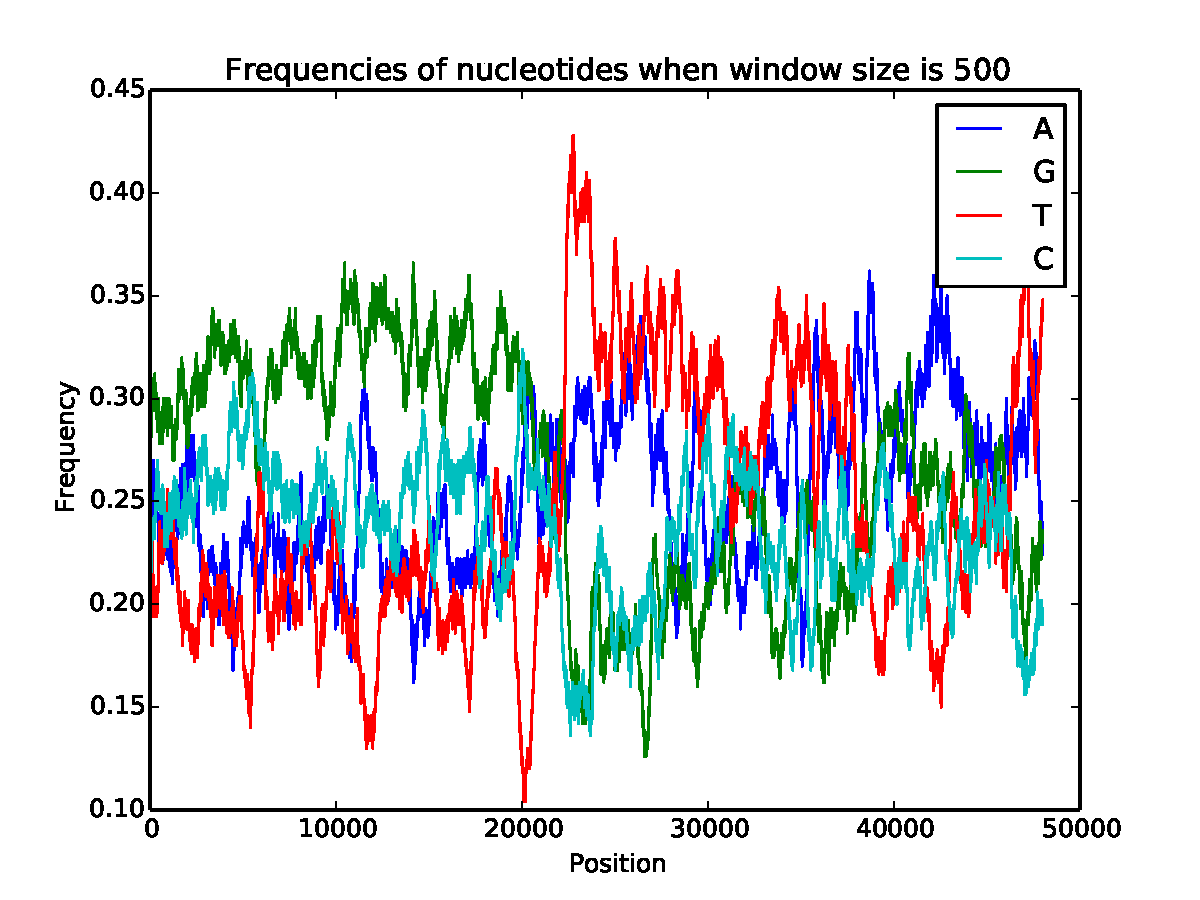
\includegraphics[width=4in]{nuc-window-500.pdf}
	\caption{Nucleotide frequences when window size is 500}
	\label{fig:n500}
\end{figure}
\begin{figure}[t]
	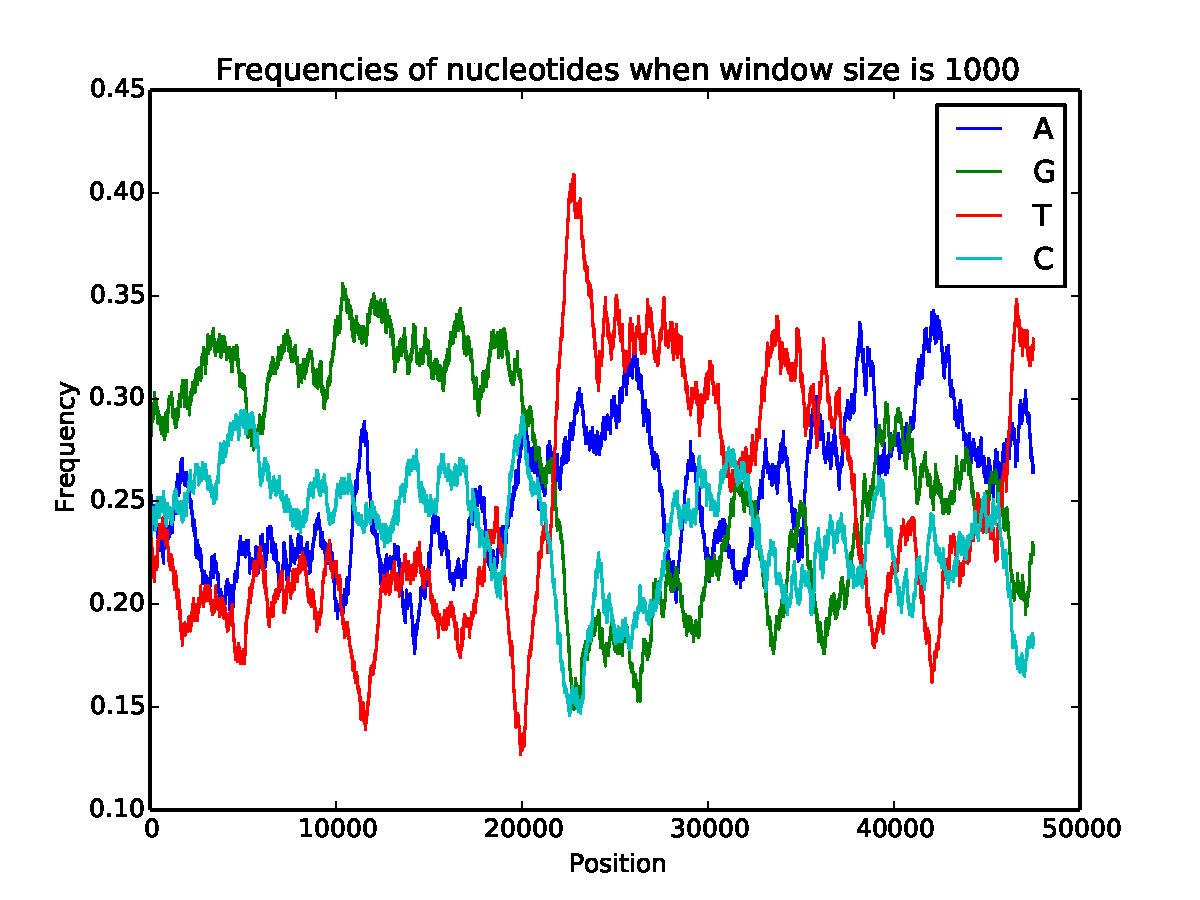
\includegraphics[width=4in]{nuc-window-1000.pdf}
	\caption{Nucleotide frequences when window size is 1000}
	\label{fig:n1000}
\end{figure}
\begin{figure}[t]
	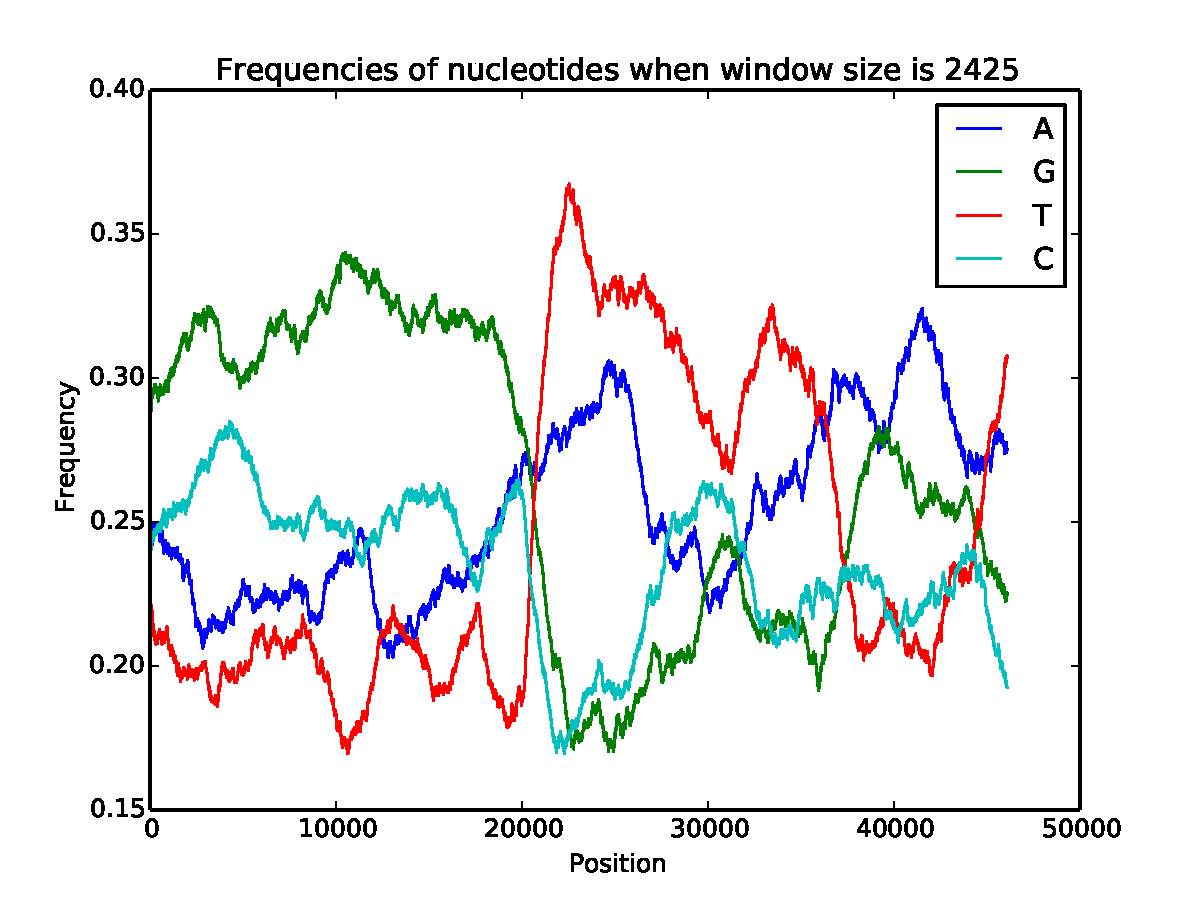
\includegraphics[width=4in]{nuc-window-2425.pdf}
	\caption{Nucleotide frequences when window size is 2425}
	\label{fig:n2425}
\end{figure}
\begin{figure}[t]
	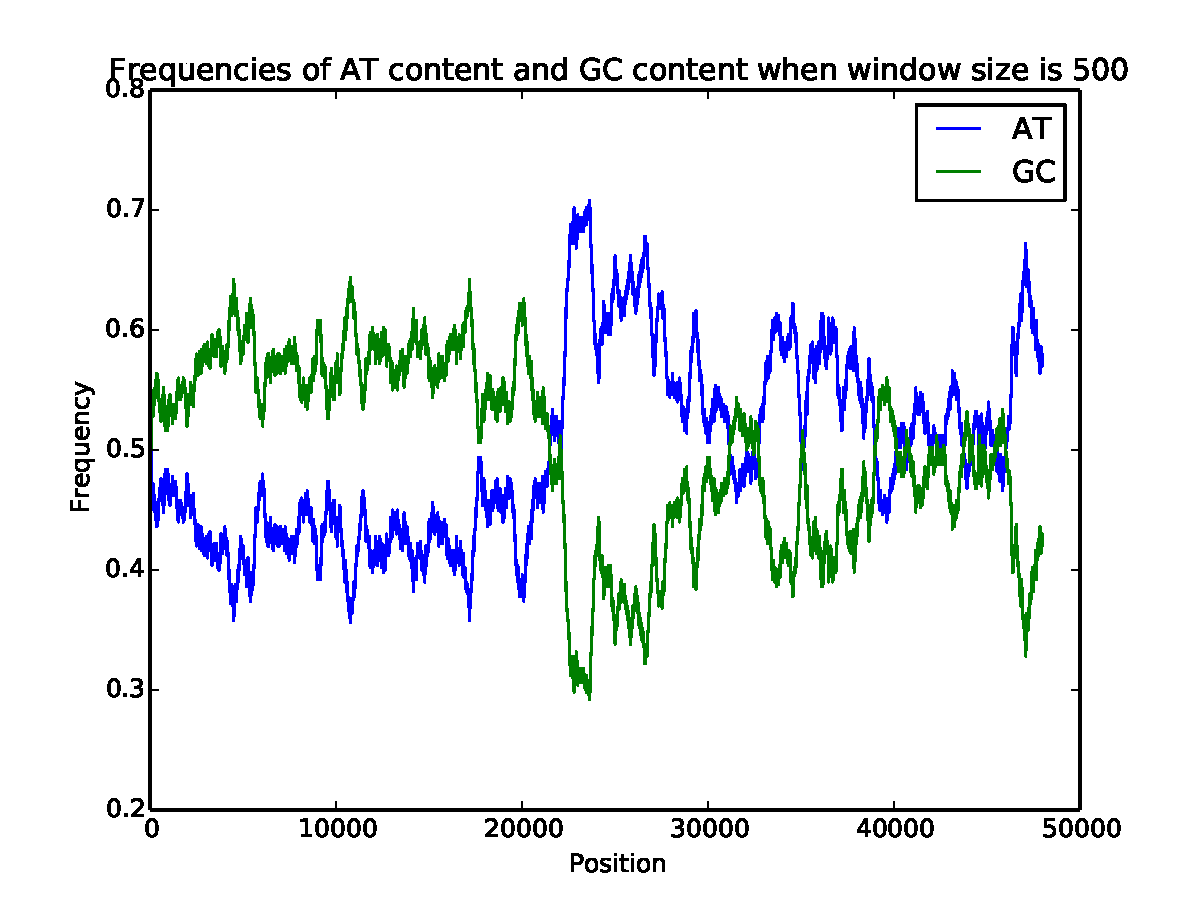
\includegraphics[width=4in]{dinuc-window-500.pdf}
	\caption{AT and CG content frequences when window size is 500}
	\label{fig:dn500}
\end{figure}
\begin{figure}[t]
	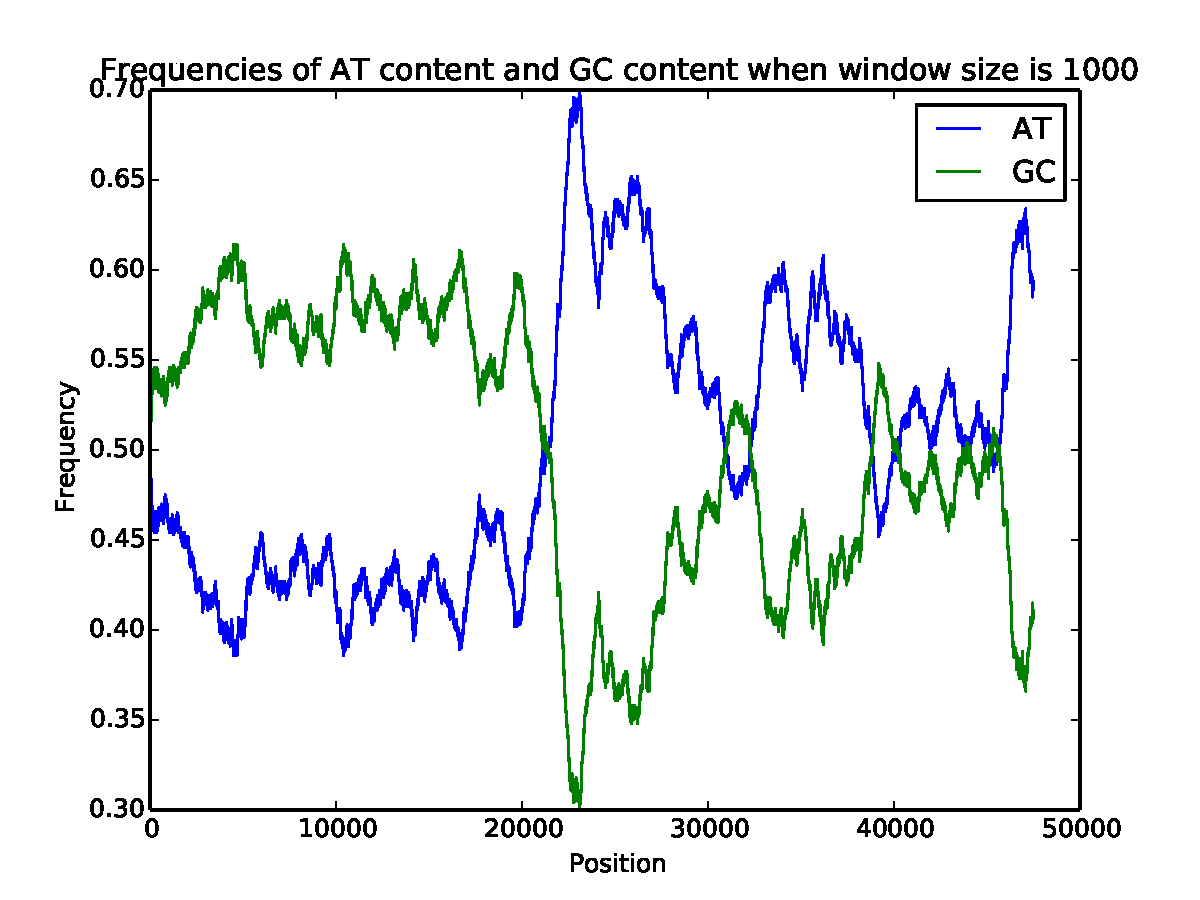
\includegraphics[width=4in]{dinuc-window-1000.pdf}
	\caption{AT and GC content frequences when window size is 1000}
	\label{fig:dn1000}
\end{figure}
\begin{figure}[t]
	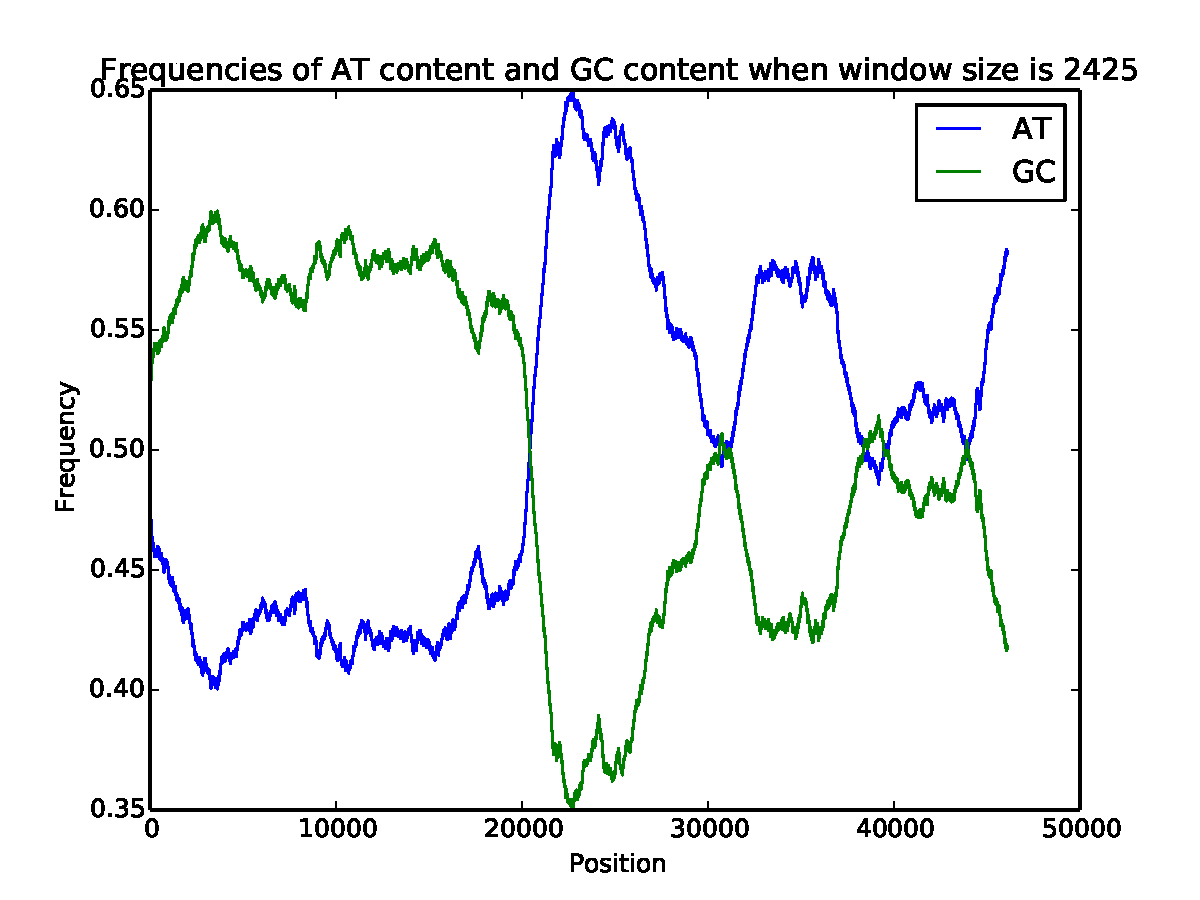
\includegraphics[width=4in]{dinuc-window-2425.pdf}
	\caption{AT and GC content frequences when window size is 2425}
	\label{fig:dn2425}
\end{figure}




%
% The following two commands are all you need in the
% initial runs of your .tex file to
% produce the bibliography for the citations in your paper.
\bibliographystyle{abbrv}
%\bibliography{sigproc}  % sigproc.bib is the name of the Bibliography in this case

% You must have a proper ".bib" file
%  and remember to run:
% latex bibtex latex latex
% to resolve all references
%
% ACM needs 'a single self-contained file'!
%
%APPENDICES are optional
%\balancecolumns

\balancecolumns
% That's all folks!
\end{document}
